% options:
% thesis=B bachelor's thesis
% thesis=M master's thesis
% czech thesis in Czech language
% english thesis in English language
% hidelinks remove colour boxes around hyperlinks

\documentclass[thesis=B,english]{FITthesis}[2012/10/20]

\usepackage[utf8]{inputenc} % LaTeX source encoded as UTF-8
% \usepackage[latin2]{inputenc} % LaTeX source encoded as ISO-8859-2
% \usepackage[cp1250]{inputenc} % LaTeX source encoded as Windows-1250

\usepackage{listings}
\usepackage{tabularx}
\usepackage{microtype}
\usepackage[htt]{hyphenat}
\usepackage[T1]{fontenc} 
\usepackage{lmodern}
\usepackage{minted}
\usepackage{float}

\usepackage{graphicx} %graphics files inclusion
%\usepackage{amsmath}
%\usepackage{xcolor}
% \usepackage{subfig} %subfigures
% \usepackage{amsmath} %advanced maths
% \usepackage{amssymb} %additional math symbols

\usepackage{dirtree} %directory tree visualisation

\usemintedstyle{friendly}
\setminted{breaklines=true}

% % list of acronyms
% \usepackage[acronym,nonumberlist,toc,numberedsection=autolabel]{glossaries}
% \iflanguage{czech}{\renewcommand*{\acronymname}{Seznam pou{\v z}it{\' y}ch zkratek}}{}
% \makeglossaries

% % % % % % % % % % % % % % % % % % % % % % % % % % % % % % 
% EDIT THIS
% % % % % % % % % % % % % % % % % % % % % % % % % % % % % % 

\department{Department of Theoretical Computer Science}
\title{Serialization of functions and environments in the R language}
\authorGN{Michal} %author's given name/names
\authorFN{Vácha} %author's surname
\author{Michal Vácha} %author's name without academic degrees
\authorWithDegrees{Michal Vácha} %author's name with academic degrees
\supervisor{Ing. Petr Máj}
\acknowledgements{I would like to thank my supervisor Ing. Petr Máj for being supportive and patient with me and my thesis. Special thanks go to other members of PRL-PRG laboratory, namely Filip Křikava and Filippo Ghibellini, who helped me many times when I was struggling with difficulties in R. Finally, I would like to thank my family and friends for their support throughout my whole studies. }
\abstractEN{This thesis is a step towards a greater endeavor: making R code more reliable and maintainable. To do that, a tool for automatic test generation called Genthat has been developed. It captures traces of function calls and then generates test cases from them. To do that is has to be able to serialize arbitrary object a function may take as an argument or return as a result. Although R is a functional language and therefore the usage of closures is abundant, they have not been supported by Genthat. In my work, I have implemented the serialization of closures and improved other areas, namely serialization of language expressions and the code clarity of generated tests.}

\abstractCS{Tato bakalářská práce je součástí větší snahy, a to udělat kód napsaný v R spolehlivější a lépe udržovatelný. K tomu byl vytvořen nástroj pro automatické generování testů, Genthat. Jeho cílem je trasovat volání funkcí a z těchto záznamů následně vytvořit sadu testů. Aby to bylo možné, je nutné, aby Genthat uměl serializovat libovolný objekt, který může funkce v R přijímat jako parametr nebo vracet. R je funkcionální jazyk, a proto se v něm často používají first-order funkce (closures), které zachytávají kontext, kde byly vytvořeny. Tyto funkce nebyly dříve v Genthatu podporovány a mým úkolem bylo přidat jejich podporu. Mimo to jsem vylepšil i ostatní části, konkrétně serializaci výrazů a čitelnost výsledných testů.}

\placeForDeclarationOfAuthenticity{Prague}
\keywordsCS{R, generování testů, funkcionální programování, serializace dat, Genthat }
\keywordsEN{R, test generation, functional programming, data serialization, Genthat}
\declarationOfAuthenticityOption{1} %select as appropriate, according to the desired license (integer 1-6)
% \website{http://site.example/thesis} %optional thesis URL


\begin{document}

% \newacronym{CVUT}{{\v C}VUT}{{\v C}esk{\' e} vysok{\' e} u{\v c}en{\' i} technick{\' e} v Praze}
% \newacronym{FIT}{FIT}{Fakulta informa{\v c}n{\' i}ch technologi{\' i}}

\setsecnumdepth{part}
\chapter{Introduction}

R is currently the most popular programming language in the field of data science and statistics \cite{ieeeTop}. As these fields are gaining momentum, so is R \cite{soTrends}. In the beginning, it has been used mostly by researchers\footnote{The precursor of R language, the S language has been developed at Bell Laboratories \cite{langS}}, but nowadays it is becoming a central part of business intelligence pipelines even at large companies like Facebook or Microsoft\cite{usingR} and the demand for reliable and maintainable R code is ever increasing. 

Genthat is an open source project\footnote{\url{https://github.com/prl-prg/genthat}} which aims to address these demands by creating tests from observed function calls such as when function f(a, b) is called with arguments 1 and 2, the following test is produced:

\begin{minted}{r}
test_that("lapply2", {
    expected <- 3L
    expect_equal(f(1L, 2L), expected)
})
\end{minted}

To do so, Genthat must know how to serialize the argument values so that they can appear in the tests. Prior to my thesis, Genthat was not able to serialize functions and therefore functions taking other functions as arguments, which is a common pattern in R and functional languages in general.

\section{Goal}
The goal is to be able to trace any call to a common function like \verb|lapply2|\cite{advR}, which accepts a function and applies it to a list.

\begin{minted}{r}
lapply2 <- function(x, f, ...) {
  out <- vector("list", length(x))
  for (i in seq_along(x)) {
    out[[i]] <- f(x[[i]], ...)
  }
  out
}
values <- list(10L, 20L, 13L, 15L, 18L)
mod <- 13L
lapply2(values, function(x) (x + 5) %% mod)
\end{minted}

And generate the following test case:

\begin{minted}{r}
test_that("lapply2", {
    expected <- list(2L, 12L, 5L, 7L, 10L)

    values <- list(10L, 20L, 13L, 15L, 18L)
    mod <- 13L

    expect_equal(lapply2(values, function(x) (x + 5) %% mod), expected)
})
\end{minted}


\section{Thesis organization}
 Chapter \ref{chap:R} describes all the nuances of the R language which are relevant in the context of Genthat and this thesis. The most important parts are about evaluation of expressions in R and how it searches for variables in the search path. The following chapter \ref{chap:genthat} is a brief overview of how the Genthat package works. Chapter \ref{chap:args} describes the work of my colleague which I have build upon and the following chapters \ref{chap:expr} and \ref{chap:clos} describe the problems I have solved as a practical part of my bachelor’s thesis. 

\section{Code samples}
This thesis includes many short code examples, typically in R. They may be just pieces of R code without output:

\begin{minted}{r}
lapply(numbers, function(x) x %% n)
\end{minted}

Or they may be written in a form of a snippet from execution of the R repl (Read-eval-print loop is a shell used for interactive programming which takes user input line by line, executes it and returns the result. The repl snippets are recognizable by \verb|>| in front of the lines, that represent user input. Lines that are not prefixed by \verb|>| represent output from the last executed statement.

\begin{minted}{r}
> exp <- function(e) pryr::sexp_type(e)
> exp(f)
[1] "CLOSXP"

\end{minted}

First two lines are inputs and the third is an output. It is a vector containing one element \verb|"CLOSXP"|. Because R indexes items from one, the index in the brackets is one. Pryr package\cite{pryr} is often used for printing R structures of properties.

\section{Genthat as a way towards an alternative R implementation}
R’s main advantage over competing products is its vast repository of existing packages. On the other hand, the main disadvantage of R is its slowness as \cite{vitek} states: ``In the Shootout benchmark R is on average 501 slower than C and 43 times slower Python. Benchmarks where R performs better, like Shootout’s regex-dna (only 1.6 slower than C), are usually cases where R delegates most of its work to C functions.'' There have been many attempts to write a faster interpreter for R.

While the alternative implementations of R like FastR\footnote{\url{https://github.com/graalvm/fastr}} or Renjin\footnote{\url{https://github.com/bedatadriven/renjin}} are indeed faster \cite{renjin}, but they lack the backwards compatibility with all the existing R code\footnote{Renjin has it's own package repository at \url{http://packages.renjin.org} and it is just a subset of CRAN repository, with many packages having their tests failing.}. 

The problem with R is that it does not have a specification\footnote{As of writing this thesis there is only a draft of the specification available} that would be compulsory for all the implementations to abide by. The official implementation of R, the CRAN-R is often called a referential implementation and if full language specification was ever made, it would describe the behavior of CRAN-R. We can compare this situation with JavaScript, which is also a dynamic interpreted language, but has a formal specification called ECMAScript\cite{EcmaScript}. Even though every browser has its own implementation of JS interpreter, works with any existing JS code, that is compliant with the ECMAScript specs. In the JavaScript world, this has enabled competition who would became the fastest between browser vendors. 

Genthat may be used to generate as many test cases for existing R code as possible, so these tests could be used to verify whether the alternative implementations of R (like FastR) are going to work correctly with existing R codebases and most importantly work with existing packages from CRAN repository\footnote{\url{https://cran.r-project.org/}}\cite{testRPoster}.

\setsecnumdepth{all}

\chapter{Introduction to R} \label{chap:R}
This chapter describes all the features of R required to understand the content of this bachelor’s thesis. It also describes some of the advanced concepts of R that are useful to understand in order to be able to think in R from a perspective of a programmer and not just a user.

\section{Objects}
Working with data in R is done using objects, they are specialized data structures, that abstract the user from working directly with the computer's memory. Objects can be used via symbols or variables they are bound to \cite{specs}.

All the relevant data types for this thesis can be found in table \ref{tab:types}. The first column of the table shows the data type as returned by the R’s \verb|typeof| function, second column is SEXP type - structure that R uses to represent the object internally and how it is seen when accessing R objects from C.

\begin{table}
	\caption[Data types in R]{Data types in R}\label{tab:types}
	\begin{tabularx}{1\textwidth}{|l|l|X|}\hline
		Type		& SEXP type		& Description \tabularnewline \hline \hline
		NULL		& \verb|NILSXP|		& Null value  \tabularnewline \hline
		Symbol	& \verb|SYMSXP|	& Name of a variable or an arbitrary symbol in a language expression.  \tabularnewline \hline
		Pairlist	& \verb|LISTSXP|	& Structure containing arguments in function declaration. \tabularnewline \hline
		Closure	& \verb|CLOSXP|	& Closure  \tabularnewline \hline
		Environment	& \verb|ENVSXP|	& Environment  \tabularnewline \hline
		Promise	& \verb|PROMSXP|	& Language expression with an environment in which it should evaluate. \tabularnewline \hline
		Language	& \verb|LANGSXP|	& Language expression  \tabularnewline \hline
		Special	& \verb|SPECIALSXP|	& Internal function that does not force evaluation of its arguments. \tabularnewline \hline
		Builtin	& \verb|BUILTINSXP|	& Internal function that does force evaluation of its arguments. \tabularnewline \hline
		Logical	& \verb|LGLSXP|	& A vector of Boolean values. \tabularnewline \hline
		Integer	& \verb|INTSXP|	& A vector of integers.  \tabularnewline \hline
		Double	& \verb|DBLSXP|	& A vector of real numbers (doubles).  \tabularnewline \hline
		Character & \verb|STRSXP| & A vector of characters, also referred to as a string. \tabularnewline \hline
		List	& \verb|VECSXP|	& A list (also called recursive vectors).  \tabularnewline \hline
		Expression	& \verb|EXPRSXP|	& A vector of language expressions.  \tabularnewline \hline
		\ldots	& \verb|DOTSXP|	& Triple dots representing arbitrary number of arguments in function. declaration  \tabularnewline \hline		
	\end{tabularx}
\end{table}

\subsection{Vectors}
Vectors represent basic data types in R, they are also called atomic vectors, because they can contain only items of basic (atomic) types: logical, integer, double, character, complex and raw\footnote{Complex and raw types differ from the rest as they cannot exist inside an unevaluated language expression. They are only mentioned for completeness and are otherwise unimportant for this thesis.}. All items inside a vector must be of the same type, hence vectors are referred to as monomorphic or homogenous data types \cite{advR}. Every item of a vector can be referred via its index and we can easily iterate over a vector’s items.

R does not have any “scalar” types. Single values are represented by vectors of length one.

To create a vector, we use the \verb|c| function as shown in the example. \verb|c| means concatenate and we can think about the \verb|c| calls as a concatenation of objects passed into in. In the following examples, they are all length 1 vectors.

\begin{minted}{r}
> c(1, 2, 3, 4)
[1] 1 2 3 4
\end{minted}

We can use \verb|typeof| function to see the data type.

\begin{minted}{r}
> typeof(c(1, 2, 3, 4))
[1] "double"
\end{minted}

It may be surprising that R returned double and not integer. This is because the implicit type of numbers in R is double\footnote{(It is usually an integer in most programming languages.)} and to get a vector of integers, we have to suffix the values with \verb|L|.

\begin{minted}{r}
> typeof(c(1L, 2L, 3L, 4L))
[1] "integer"
\end{minted}

\subsubsection{Coercion of atomic types}
Another aspect of vectors is type coercion. That means that when values of distinct types are passed to \verb|c|, R would not show an error because vectors are monomorphic, but instead it coerces all the passed values into the most flexible type. For example, if we try combining integers and real numbers, we get a vector of doubles, because we can take any integer and represent it as a double, but not the other way around (hence double is more flexible than integer).

\begin{minted}{r}
> typeof(c(1L, 2, 3, 4))
[1] "double"
\end{minted}

We can easily coerce logical values to integers, integer to doubles and doubles to strings. That means if any of the value passed to \verb|c| is a string (and the rest logical, int and doubles), we get a vector of strings.

\subsection{Lists}
Lists are made of items, each of which can be of different R type. That means lists are heterogenous (also called polymorphic) data structures\cite{advR}. Lists can be used to store data types, which cannot be stored in vectors, like functions or other lists. Lists are also called recursive vectors, because they can contain other lists. To create a list, we use the \verb|list| function.

\begin{minted}{r}
> list(1, list(2, "3"))
[[1]]
[1] 1

[[2]]
[[2]][[1]]
[1] 2

[[2]][[2]]
[1] "3"
\end{minted}

\subsection{Language expressions}
Language objects represent unevaluated parsed R code. Their form is an AST (abstract syntax tree) which is made of four different node types: calls, names, constants and pairlists. Although R has a special type called expression (that behaves like a list of language objects), when the word expression is used, it refers to the language expression (This follows convention from \cite{advR}).

Language objects enable us work with the expressions themselves (the parsed R code) and not just its result. The distinction should be obvious from this example:

\begin{minted}{r}
> y <- 1
> x <- y + 2
> x
[1] 3
\end{minted}

Variable \verb|x| contains the result of an expression \verb|y + 2|. This expression is evaluated immediately when it is assigned to \verb|x|, so \verb|x| never contains the expression, only the result.

\begin{minted}{r}
> y <- 1
> x <- quote(y + 2)
> x
y + 2
\end{minted}

Encapsulating the expression in a \verb|quote| function call, preserves the expression and does not evaluate it. We can now say that \verb|x| contains a quoted expression\cite{advR} of \verb|y+2| to emphasize that the expression is not evaluated. 

Having the expression itself and not just the result enables us to perform computation on the language itself (also called metaprogramming), as we are able to modify the expression during runtime of our program or evaluate it in arbitrary environment.

\subsection{Function objects}
In R, you can work with functions as with any other objects, they can be assigned to variables or passed and returned from other functions. A function in R has three basic parts: formals, body and environment. 

Formals is a list of argument names and their default value. Ellipsis (\ldots) used as an argument name have a special semantics as they represent ability to accept arbitrary number of arguments. 

Environment is a reference to the environment where the function should look for values of symbols that are not arguments or local variables. It is also called an enclosing environment or a captured environment. Function with a captured scope (environment) is a closure, so in R every function except for special and builtin functions is a closure.

In it is R possible to read and modify all three parts of a function.

\subsubsection{Builtin and special functions}
Both types represent built-in functions in R, which are core functions of R implemented in C. They do not have any body, formals or environment associated with them, because they do not contain any R code. The difference between \verb|builtin| and \verb|special| is how they evaluate their arguments. Special functions do not force evaluation of their arguments, builtins do.

For example the already mentioned \verb|quote| function is a special object, because it needs to work with the unevaluated expressions. 

\begin{minted}{r}
> typeof(quote)
[1] "special" 
\end{minted}

The example of builtin function can be a plus operator, that requires its arguments to be evaluated, because we want to compute the addition of two numbers and not the symbols that may be contain the values.

\begin{minted}{r}
> typeof(`+`)
[1] "builtin" 
> a <- 1
> b <- 5
> quote(a + b)
a + b
> a + b
[1] 6 
\end{minted}

\subsection{Promises}
Promise is a special object, that encapsulates an R expression, which gets lazily evaluated. That means it is not evaluated when assigned to a variable, but when the variable gets read for the first time, the expression gets evaluates and then the result is cached. All the subsequent reads of the variable just return the cached result. The act of evaluating a promise for the first time is called forced evaluation \cite{specs}. 

Because the contexts when promise is created and when it is called for the first time may differ, there is also an environment associated with it. The environment tells the promise object in which environment it should evaluate the encapsulated expression.

When a function is called its arguments are matched and then each of the formal arguments is bound to a promise (for functions supporting arbitrary number of arguments also all of the unmatched names are bound to the promises). The expression that was given for the specific argument and a reference to the environment the function was called from are stored in the promise \cite{specs}. The reason behind this behavior is that now a function can decide whether it will work with the value or the expression passed to it. To extract the expression of the promise R has the function \verb|substitute|, which returns a language expression. Working with arguments by using their expressions and not values is called a non standard evaluation \cite{advR}.

There is one more way to create a promise except when passing argument to a function and that is by calling function \verb|delayedAssign| instead of using assign or assignment operator \verb|<-| when binding variable and its value/expression.

Following example shows simple function \verb|f|, that accepts two parameters \verb|a, b|, but only works with \verb|b|. Therefore \verb|a| never gets evaluated and even if we pass unexisting variable for \verb|a| it does not show an error.

\begin{minted}{r}
> f <- function(a, b) b
> f(notFound, 10)
[1] 10
> f(10, notFound)
Error in f(10, notFound) : object 'notFound' not found
\end{minted}

\section{Environments}
Understanding of environments is a precursor to understanding the more advanced topics in R and it is essential to grasp their meaning in order to reason about computing on the language itself and tracing the function calls that Genthat is all about.

\subsection{Structure of an environment}
As mentioned previously environment is where the promises get evaluated and where R finds stuff. Environment is a data structure that enables scoping in R. It is comprised of a symbol-value pairs and a reference to the parent environment. Sometimes the symbol-value pairs are also called the environment’s frame. When R looks up a symbol value in an environment it first checks the symbol-value pairs and if it is not found there, it recursively continues the search to the parent environment until the symbol is found or the empty environment is reached. Empty environment represents the end of environments hierarchy and has no parent.

\subsection{Parent environment}
Every environment contains a reference to a parent environment (also called an enclosing environment). In the following scenario \verb|e1| is the parent of \verb|e2| (visualized with the dashed arrow).


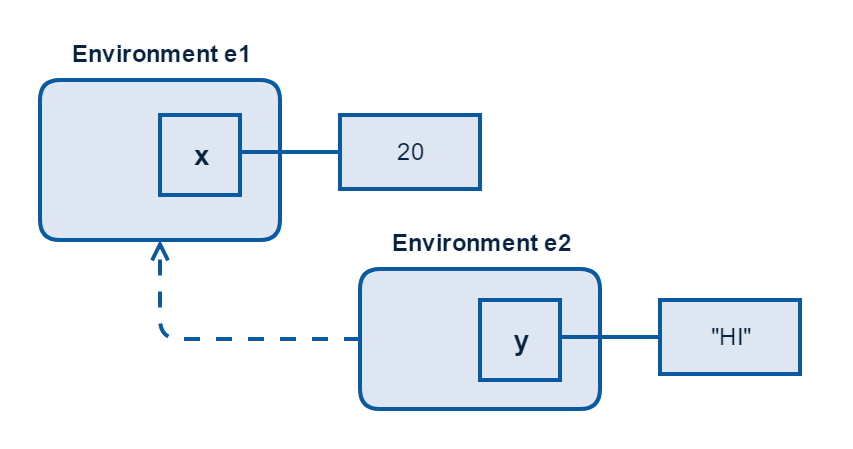
\includegraphics[width=0.75\textwidth]{img/parent-env.png}


When we try to evaluate the symbol \verb|x| in \verb|e2| we receive the value 20 from the parent environment. But it doesn’t work the opposite way – \verb|e1| does not know about \verb|e2|’s existence and therefore we cannot get the value of \verb|y| from it. The hierarchy of environments where we look for the symbol is also called the search path \cite{specs}.

\begin{minted}{r}
> eval(quote(x), e1)
[1] 20
> eval(quote(x), e2)
[1] 20
> eval(quote(y), e1)
Error in eval(expr, envir, enclos) : object 'y' not found
> eval(quote(y), e2)
[1] "HI"
\end{minted}

\subsection{Environment hierarchy}
The previous example was really simplistic, when R repl starts up or an R script is executed, the execution begins in the global environment (named \verb|.GlobalEnv|), that already has a hierarchy of parent environments. They can be printed by calling the \verb|search| function.

\begin{minted}{r}
> search() # prints current search path
[1] ".GlobalEnv" "package:stats" "package:graphics"
[4] "package:grDevices" "package:utils" "package:datasets"
[7] "package:methods" "Autoloads" "package:base"
\end{minted}

This is how the hierarchy looks like (bindings from symbols to values are omitted for brevity):

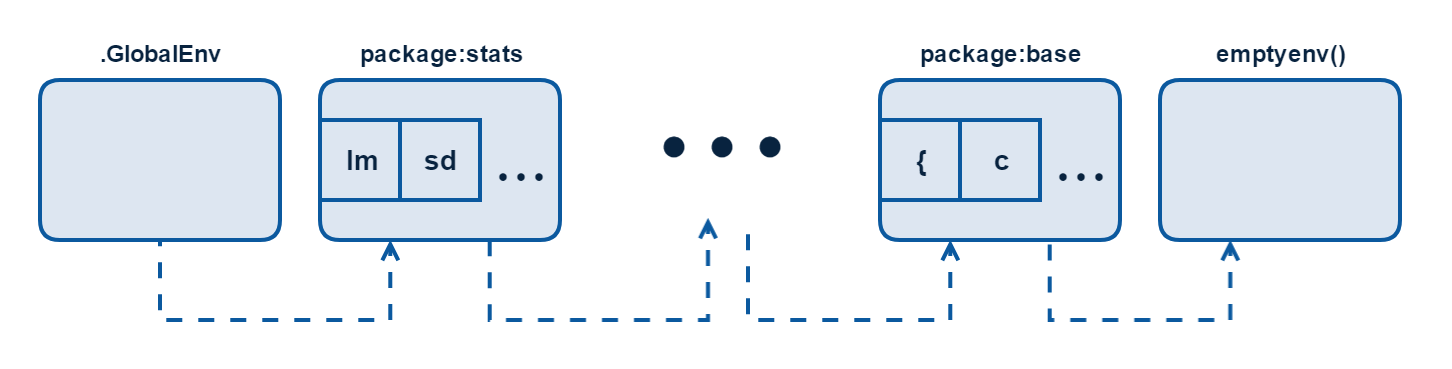
\includegraphics[width=\textwidth]{img/search-path.png}

All the package environments represent loaded packages, which are available to use for the running R code. Every call to \verb|library(packageName)| adds a \verb|package:PackageName| environment into the search hierarchy just after the global environment.

Inside the \verb|package:stats| environment there are symbols \verb|lm|, \verb|sd| and in the \verb|package:base| there is the left bracket and \verb|c| function. All of these are R functions and because they are in the search path from the beginning, they can be used without manually loading any packages. The \verb|emptyenv()| represents empty environment, that has no parent nor any symbols in it.

\subsection{Binding and enclosing environments}
It has been already mentioned that every function has an environment it encloses and every variable is bound in an environment. To get a better perspective of it, here is a simple example of a function that is bound in the global environment and also encloses it.

\begin{minted}{r}
> x <- 1
> f <- function() x
\end{minted}

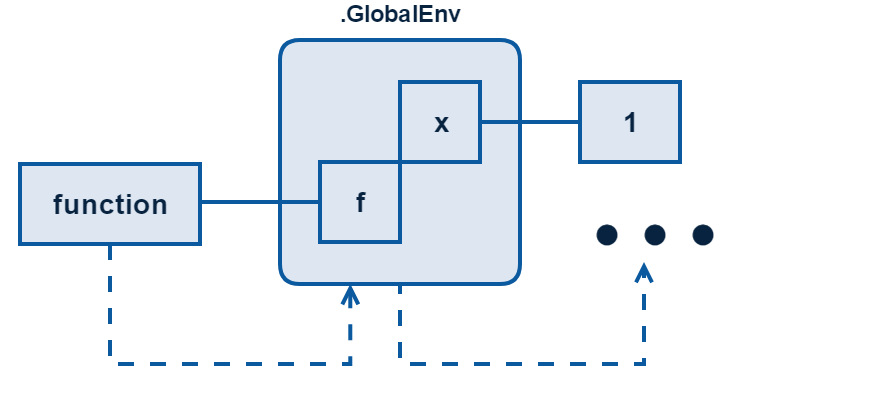
\includegraphics[width=0.7\textwidth]{img/enclosing-binding.png}

\begin{minted}{r}
> environment(f) #prints the enclosing environment of f
<environment: R_GlobalEnv>
\end{minted}

\subsection{Package environments}

Values can have more than one binding environment and R uses that for functions that are exported (made public) from packages. All the exported functions are bound in the \verb|package:packageName| environment. There are another two environments that R creates for each package:  \verb|package:namespace| environment and \verb|imports| environment. Namespace environment binds all the functions of the package (not just the exported ones) and its parent is the import environment for the package. The import environment binds all the exported symbols from the dependent packages.

The following example \ref{fig:hierarchy} shows the environment hierarchy after the Genthat package has been loaded. Genthat depends on the \texttt{codetools} package\cite{codetools}, so its exported functions are also bounded in its imports environment, but the enclosing environment of \texttt{findGlobals} is still the same – it’s the \texttt{namespace:coodetool} environment. The last unmentioned environment is \texttt{namespace:base}. \texttt{Namespace:base} contains binds for allexported functions in the \texttt{package:base} and its parent environment is \texttt{.GlobalEnv} and all the imports environment encloses it.

\begin{figure}\centering
    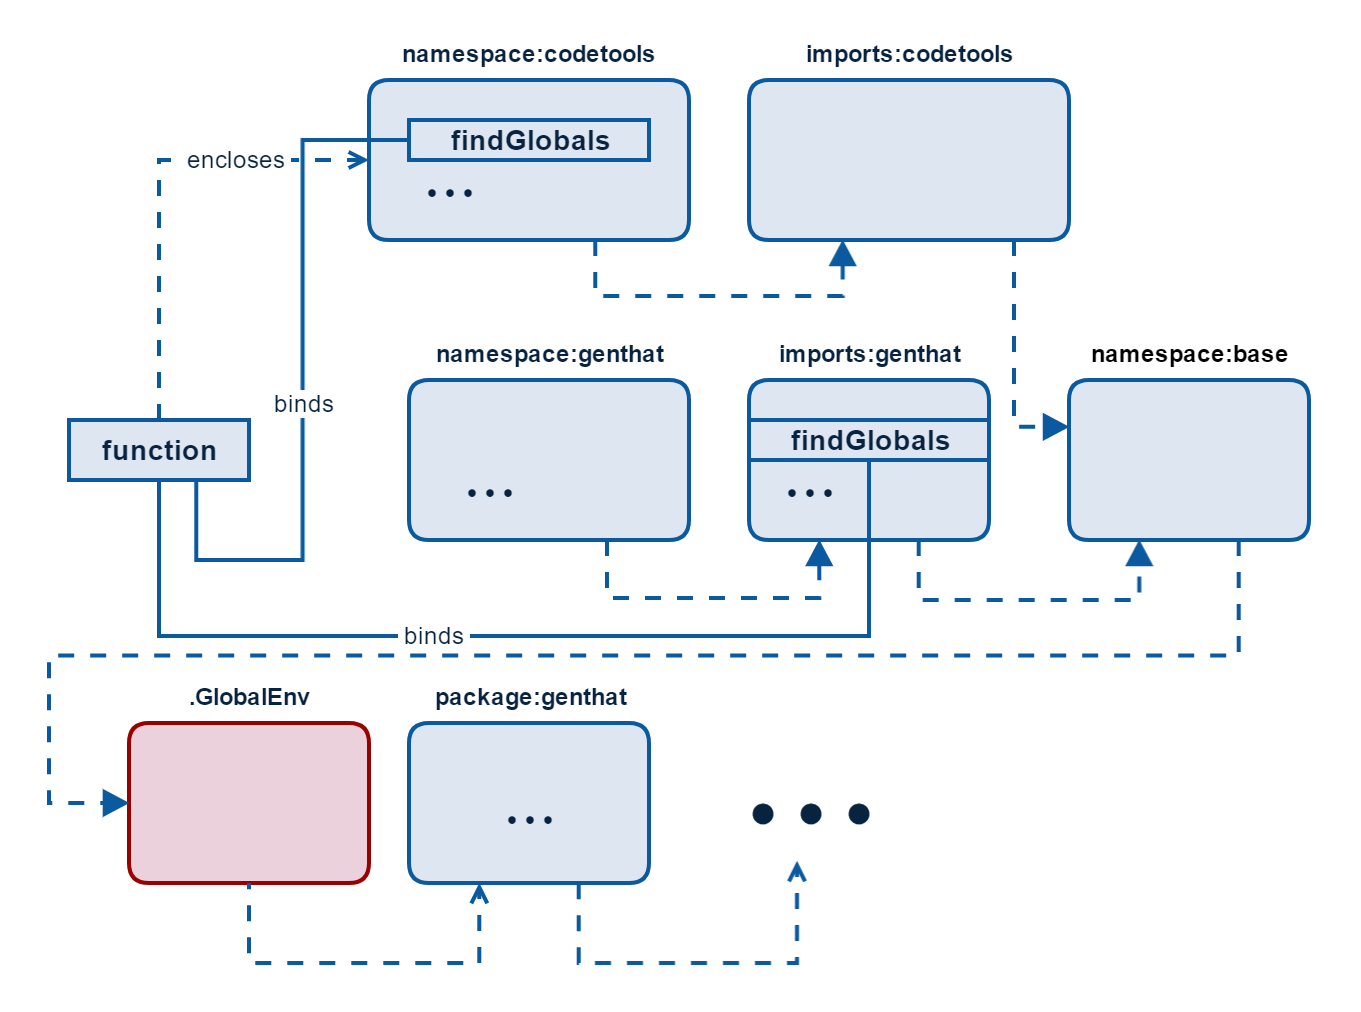
\includegraphics[width=\textwidth]{img/hierarchy.png}
	\caption[Example hierarchy of environments in R]{Example hierarchy of environments in R}\label{fig:hierarchy}
\end{figure}

\subsection{Execution environment}
When a function is called a new environment is created for its run. At first all the arguments are copied to it in a form of promises and its parent environment is set to the enclosing environment of the function. Every local variable the function declares also goes to its execution environment. After the function is finished, the execution environment goes away unless there is a closure that captures is and escapes (e.g. by being returned from the function). 

\subsection{Calling environment}
R also has a special term for the environment from which the function was called: the calling environment. The most important thing about this environment is that arguments (passed in the form of promises) are evaluated in this environment. They are bound in the newly created execution environment of the called function, but evaluated in the calling environment.

\section{Scoping}
Scoping tells us how and where R looks for values of different symbols.

\section{Lexical scoping}
When a function needs a value of a symbol that is not an argument or a local variable, it uses lexical scoping. That means R looks into the enclosing environment and then its parent environments.

There are two rules that are essential about lexical scoping: \\
It distinguishes between variables and functions, so assigning a value to symbol \verb|c|, does not break the subsequent calls to the function \verb|c|.

\begin{minted}{r}
> c <- 10
> c(c)
[1] 10
\end{minted}

Second is that the lookup is dynamic, if a function references a symbol from the enclosing scope and the value of the symbol changes between two calls of the function, it returns two different results.

\begin{minted}{r}
> add5 <- function() c + 5
> add5()
[1] 15
> c
[1] 10
> c <- 100
> add5()
[1] 105
\end{minted}

\subsection{Dynamic scoping}
Dynamic scoping means looking up variables in the calling environment instead of the enclosing environment. Function can get the calling environment by calling \verb|parent.frame()| and when it evaluates an expression in it, it is said it uses dynamic scoping. If the calling and enclosing environments are the same, we get the same result as if lexical scoping is used. But this is not very typical. Usually dynamic scoping is used by functions that are exported from a package (so their enclosing environment is not our calling environment) that either manipulate or look into the environment from which they were called from.

\section{Closures}
Although every function that has an environment associated with it is a closure, the name closure is often used just for functions returned from another function (and therefore enclosing the execution environment of the parent function) \cite{advR}. It is not considered good practice to reference variables from the global environment \cite{advR}, on the other hand capturing the execution environment of parent function can be beneficial as it enables us to create factory functions and to manage the mutable state.

\subsection{Factory functions} \label{ssec:clos1}
Factory functions are functions, that create a function based on the arguments passed to it. They are useful when regular function would require many arguments, that would be the same across different calls or when they use some of the arguments for initialization, that needs to be done only once and can be expensive in terms of I/O access or CPU time. Following example is intentionally simplistic only to describe this pattern and does not represent best practice when it should be used.

Mod adder is a factory function for creating add functions in modular arithmetic. It returns a new function that takes two operands \verb|(a, b)| and adds them in the specified module mod.

\begin{minted}{r}
> mod_adder <- function(mod) function(a, b) (a + b) %% mod
> add5 <- mod_adder(5)
> add13 <- mod_adder(13)
\end{minted}

The bodies of both closures \verb|add5| and \verb|add13| are the same, but their environments differ.

\begin{minted}{r}
> add5
function(a, b) (a + b) %% mod
<environment: 0x000000001d22aeb0>
> add13
function(a, b) (a + b) %% mod
<environment: 0x000000001d1fb9d0>
\end{minted}

The captured execution environments contain the mod argument passed to the original factory function.

\begin{minted}{r}
> ls.str(environment(add5))
mod :  num 5
\end{minted}

\subsection{Managing the mutable state} 
In R functions can modify (mutate) variables in their enclosing environment by calling the scoping assignment operator \verb|<<-|. When mutating variables in the enclosing scope (e.g. the global environment) there is a risk that another function may mutate the variable we are using to store the function’s state and thus inadvertently affect the execution of our function. Closures solve this by encapsulating the state in the captured execution environment of the parent function. Following example shows a simple modular counter.

\begin{minted}{r}
> mod_ctr <- function(mod) {i = 0; function() {i <<- (i + 1) %% mod; i}}
> ctr3 <- mod_ctr(3)
> ctr3_2 <- mod_ctr(3)
> ctr3()
[1] 1
> ctr3_2()
[1] 1
> ctr3_2()
[1] 2
> ctr3_2()
[1] 0
> ctr3()
[1] 2
\end{minted}

The example shows, that the state of the both counters is isolated and cannot be inadvertently mutated by another function call.

\chapter{Genthat} \label{chap:genthat}
\section{How R community may use Genthat}
Genthat may help package creators with the adoption of unit testing inside their packages. Many packages in the CRAN repository usually have a sample of their usage in files called vignettes. These vignettes are in the RMarkdown format and contain code snippets describing how to use the package. We could use the snippets to generate tests for the package and then the author may include them with the other unit tests for the package to make sure he has not broken any of the package’s main functionalities before he submits an updated version to the repository.

\section{How Genthat works}
\subsection{Function decoration (instrumentation)}
First step in order to generate tests is to decorate the functions we want to generate the tests for. This is done using the \verb|decorate_functions| call. Functions can be decorated individually or in bulk when using the package argument to decorate all the functions inside a package

\begin{enumerate}
\item Decorate a single function.
\begin{minted}{r}
>decorate_functions("fn1")
\end{minted}
\item Decorate all the functions a package exports.
\begin{minted}{r}
>decorate_functions(package = "somePackage")
\end{minted}
\item Decorate all the functions in a package including non-exported ones.
\begin{minted}{r}
>decorate_functions(package = "somePackage", include_hidden = TRUE)
\end{minted}
\end{enumerate}

The \verb|decorate_functions| instruments the functions by creating a new body containing first the Genthat’s instrumentation code and then the original body, it also adds a trigger to the \verb|on.exit| hook, which runs every time the function execution is finished. The body of the original function is then replaced by the newly created one.

The code in the functions’ beginning handles the tracing of their arguments and the \verb|on.exit| trigger traces the returned value.

\subsection{Tracing the function calls}
After the function has been decorated, every call to it is captured and creates a trace. When the trace is created all of its content is serialized in a way that makes it easy to generate tests from it.

\subsection{Serializing R structures into R code}
There are few ways how to serialize objects in R. The first is by calling the \verb|serialize| function in R. This supports serialization of any R object, but the downside is that it serializes it into a binary format. Using this for test generation is not an option, because we want the tests to be as readable as possible. Another option is serializing to JSON/XML or any typical data exchange format. They are suitable for their readability and that people are familiar with them. The downside is that these serializers do not support serialization of arbitrary R objects, they support only the basic data types R uses for working with data (lists, vectors, data.frames…).

Genthat went with custom serialization written in C++, that serializes R objects into the R code. It is not typical, but it satisfies the condition of serializing arbitrary R object, making human readable output and generating tests that would be easily editable.

There are two different methods to serialize R objects: \verb|serialize_r| and \verb|serialize_r_expr|. The second method is used for serializing language expression objects in R that are in a context where they do not have to be enclosed in quote function, typically arguments of a function call. \verb|Serialize_r| is used in all other cases and it only calls \verb|serialize_r_expr| when it needs to serialize a nested language expression or an item in a pairlist. \\ \verb|Serialize_r_expr| is also simpler, because some types cannot exist inside a language expression (e.g. complex numbers) and all the vectors have length 1.

\subsection{Test generation}
After the trace has been serialized, it is in a form from which tests can be made easily. Function \verb|get_tests| generates tests into an output directory. It creates one file per test case and one test case per trace. 

\begin{minted}{r}
gen_tests(output_dir = "./genthat_tests")
\end{minted}

The generated tests use package \verb|testthat|\cite{testthat}, that uses syntax that is accessible and understandable even for novice users. Each test is wrapped in a \verb|test_that| function and for assertion functions with clear names like \verb|expect_identical| or \verb|expect_equal| are used.

For example for function call \verb|add13(5L, 10L)| of function \verb|add13| from the chapter \ref{ssec:clos1} Genthat would generate the following test:

\begin{minted}{r}
test_that("add13", {
    expected <- 2L

    expect_equal(add13(5L, 10L), expected)
})
\end{minted}

\chapter{Serializing arguments as expressions} \label{chap:args}
This chapter describes work of my colleague Filippo Ghibellini on serializing arguments as expressions and because I have built my work on top of it, it is essential to briefly describe it.

Genthat originally serialized only the forced values of arguments. For function call with one variable in it:

\begin{minted}{r}
x <- 10
f(x)
\end{minted}

Genthat would serialize this as \verb|f(10)|. From the function’s point of view this is the same, as long as the function is referentially transparent. Referentially transparent function behaves the same if we replace its arguments by their values. \verb|f(10)| must be the same \verb|f(x)|. But referential transparency does not hold for functions that use non-standard evaluation. Example may be the \verb|hist| function. The following call takes 1000 samples from normal distribution and prints its histogram as figure \ref{fig:hist1} shows.

\begin{minted}{r}
x <- rnorm(1000)
> hist(x)
\end{minted}

\begin{figure}\centering
    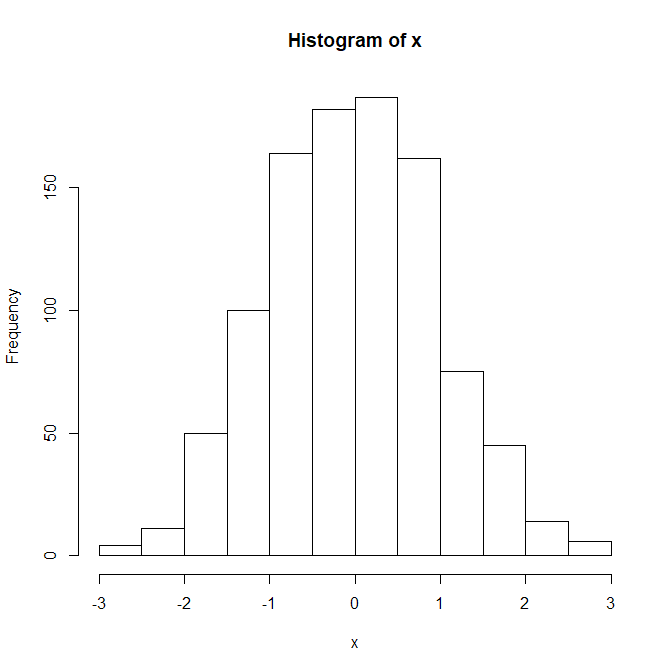
\includegraphics[width=0.7\textwidth]{img/hist.png}
	\caption[Result of calling hist with expression x]{Result of calling hist with expression x}\label{fig:hist1}
\end{figure}

As shown in \ref{fig:hist1} R used both the value and the expression \verb|x| to print this chart. If we would take the value of \verb|x| and substitute it directly into the \verb|hist| call, the resulting chart is the same, but title and \verb|x| axes label do not make sense, as figure \ref{fig:hist2} shows.

\begin{figure}\centering
    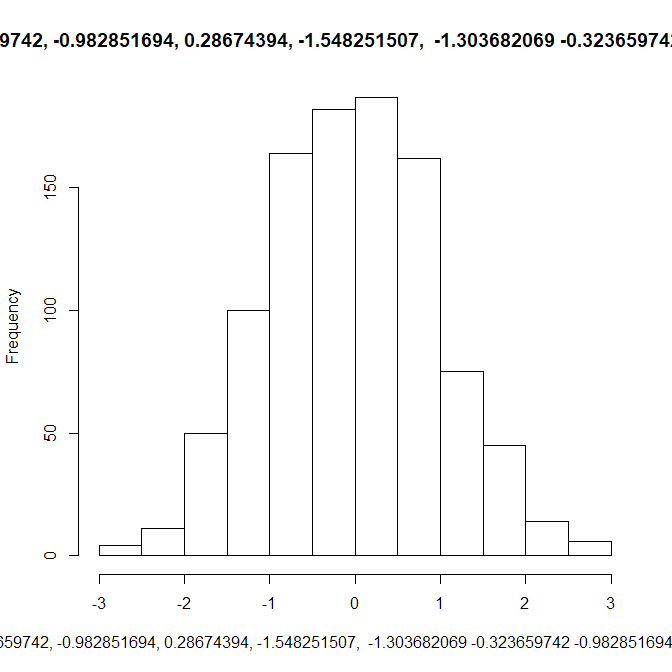
\includegraphics[width=0.7\textwidth]{img/hist2.png}
	\caption[Result of calling hist with vector of values instead of expression x]{Result of calling hist with vector of values instead of expression x}\label{fig:hist2}
\end{figure}

This is caused by \verb|hist| being referentially opaque (opposite of referentially transparent) and although the values are the same, the expressions that created them differ and \verb|hist| accesses both the value and expression for the first argument and it prints different labels for different expressions.

For correct serialization of functions like this, Filippo devised, that Genthat would be tracing both the expressions passed as argument and all the values of variables contained in those expressions.

\subsection{Capturing arguments in decorated functions}
When function is decorated, its code gets instrumented and genthat’s code is inserted before its original body and into the \verb|on.exit| handler.

The code inserted in the beginning is responsible for capturing expressions of arguments. It first gets the whole function call (by calling the \verb|sys.call()|) function in form of a list. First item of the list is the name of the function, subsetting the list by -1 removes it. This returns the arguments as unevaluated expressions. By serializing the \verb|call_args| variable we are able to recreate the function call later when generating tests.

\begin{minted}{r}
call_args <- as.list(sys.call())[-1]
\end{minted}

Second to serialize all the values for variables and functions, we must extract all the symbol names from the expressions.

\begin{minted}{r}
exprs <- as.character(c(lapply(call_args, all.names), recursive = TRUE))
\end{minted}

Then the symbol names are filtered, because they contain parenthesis, operators, keywords and other stuff that we do not have to serialize and are always available in R. 
Note: This filtering is not sufficient to cover all cases where we do not have to capture the variable value. For example it does capture variables from packages, which is not necessary. An improved filtering of names is development as of finishing this thesis.

\begin{minted}{r}
filter <- function(x)!(x %in% genthat:::operators || x %in% genthat:::keywords)
exprs <- unique(Filter(expr_ filter, exprs))
\end{minted}

Then we have to get all the values for the filtered names. Genthat uses dynamic lookup for it, because the expressions are bound in the calling environment (returned by \verb|parent.frame()| function).

\begin{minted}{r}
elem_vals <- lapply(exprs, function(name) get(name, parent.frame()))
names(elem_vals) <- exprs
\end{minted}

The variables \verb|call_args| and \verb|elem_vals| are then used to create the trace of the function call. Later when \verb|generate_tests| function is called, the trace is used to create the test case for the function.

\subsection{Test generation}
For simple example of test generation using the improvements mentioned in this chapter we are going to use a modified version of function \verb|add13| from the chapter \ref{ssec:clos1}. The modified version prints the expressions a and b passed to it, followed by the result.

\begin{minted}{r}
add13p <- function(a, b){
	print(paste0(deparse(substitute(a)), " + ", deparse(substitute(b)), " = ", (a+b) %% 13))
}
\end{minted}

\verb|Substitute| function takes the function argument and replaces it with the expression passed into the function call. \verb|Deparse| function takes a language expression and prints it as a string.

\begin{minted}{r}
>gentgat::decorate_functions("add13p")
> a <- 5L
> b <- 15L
> add13p(x, y)
[1] "x + y = 7"
\end{minted}

Function \verb|add13| is decorated, so the call is traced and the trace contains both the arguments expressions and their values:

\begin{minted}{r}
[1] "list(call=list(\"x\",\"y\"), vals=list(x=5L,y=15L), cls=list())"
\end{minted}

Calling the Genthat’s function \verb|gen_tests| transforms it into the following test case:

\begin{minted}{r}
test_that("add13", {
    expected <- "x + y = 7"

    # variables used in arguments
    x <- 5
    y <- 15

    expect_equal(add13p(x, y), expected)
})
\end{minted}

As shown above, Genthat is now able to capture calls of functions which use non standard evaluation, capture both the expressions for arguments and the values for all variables referenced in them.  The resulting test generated is as close as possible to the original function call and is easily readable. 

\chapter{Serialization of language expressions} \label{chap:expr}
\section{Previous state}
Genthat already supported serialization of simple language expressions, but before we went from forcing the function arguments to not forcing them they were not the main focus, because they would only be used in two scenarios:  first when quoted language expression and second when formula was passed to the function. 

\begin{minted}{r}
> f <- function(exp) typeof(exp)
#quoted language expression
> f(quote(a + b))
[1] "language"

#formula
> f(a ~ a + b)
[1] "language"
\end{minted}

But when we started to handle all arguments as expressions, the scope of usage has broadened and some improvements had to be done so we would be able to serialize as many language expressions as possible.

\section{Structure of language expression in R} \label{sec:ast}
Laguage expression in R is represented by its AST (abstract syntax tree) and we can use the ast() function from pryr package to print it \cite{advR}.

\begin{minipage}{\linewidth}
\begin{minted}{r}
> pryr::ast(a <- f(x) + b)
\- ()
  \- `<-
  \- `a
  \- ()
    \- `+
    \- ()
      \- `f
      \- `x
    \- `b
\end{minted}
\end{minipage}

The tree consists of four possible node types: constants, names, calls and pairlists.

\subsection{Constants}
Constants are atomic vectors with length one. They are directly represented by their values, because R optimizes the AST and does not store the expressions that creates constants. Types mentioned in table \ref{tab:astConstants} are represented as constants in the AST.

\begin{table}[h]\centering
	\caption[Constants in language expressions]{Constants in language expressions}\label{tab:astConstants}
	\begin{tabular}{|l|l|l|} \hline
        Type & SEXP type & Example values \tabularnewline \hline \hline
        Null value & \verb|(NILSXP)| & NULL \tabularnewline \hline
        Logical values & \verb|(LGLSXP)| & TRUE, FALSE, NA\tabularnewline \hline
        Integers & \verb|(INTSXP)| & -1L, 5L, \ldots, \verb|NA_integer_|\tabularnewline \hline
        Real numbers & \verb|(REALSXP)| & 1, 1.1, 5, \ldots\tabularnewline \hline
        Strings & \verb|(STRSXP)| & "a", "world", \ldots\tabularnewline \hline
    \end{tabular}
\end{table}

\begin{minted}{r}
> pryr::ast(NULL)
\- []
> pryr::ast(TRUE)
\-  TRUE
> pryr::ast(1L)
\-  1L
> pryr::ast(1)
\-  1
> pryr::ast("a")
\-  "a"
\end{minted}

Because constants are represented directly by their values, the quoted expressions that creates them and their values are identical.

\begin{minted}{r}
> identical(1, quote(1))
[1] TRUE
> identical("a", quote("a"))
[1] TRUE
> identical(TRUE, quote(TRUE))
[1] TRUE
\end{minted}

\subsubsection{Real constants}
When working with real numbers\footnote{In this thesis the numbers that would get serialized into binary form are for readability purposes presented in their textual form (e.g. 0.1)} this means that we could lose precision when extracting numbers from the AST, the internal representation of numbers uses float arithmetic and therefore its precision is limited.

The first example shows number 0.1 (number that does not have terminate decimal expansion in binary base) first as entered by the user "0.1" and then how R stores it internally (imprecise after first seventeen decimal places).

\begin{minted}{r}
> sprintf("%.20f",0.1)
[1] "0.10000000000000000555"
\end{minted}

\begin{minted}{r}
> sprintf("%.40f",3.5)
[1] "3.5000000000000000000000000000000000000000"
\end{minted}

To work around the differences in precision for different numbers and therefore possible loss in accuracy when serializing them, Genthat serializes the binary values of the numbers and then recreates the numbers from them and not from their textual representation. Because the binary format is unreadable, I have added the textual representation in the comment that's part of the trace.

The number 0.1 gets serialized as:

\begin{minted}{r}
> genthat:::serialize_r(0.1)
"readBin(as.raw(c(0x9a,0x99,0x99,0x99,0x99,0x99,0xb9,0x3f)), n=1, \"double\") #0.1\n"
\end{minted}

\subsection{Names}
Names are also called symbols in the AST they represent everything that is not a constant, call or a pairlist, so function names, keywords, variable identifiers, operators, etc.\ldots are all represented by name nodes.

In the output of the \verb|ast| function they are prefixed with a backtick.

\begin{minted}{r}
> pryr::ast(x)
\- `x
> pryr::ast(fx)
\- `fx
> pryr::ast(`+`)
\- `+
> pryr::ast(`for`)
\- `for
\end{minted}

\subsection{Calls}
Function calls are represented by call nodes. They start with pair of parenthesis followed by the function name (represented by a name node) and then all the arguments passed in the call.

\begin{minted}{r}
> pryr::ast(func(a=1,b))
\- ()
  \- `func
  \-  1
  \- `b
\end{minted}

\subsection{Argument names} \label{ssub:tags}
As shown in the previous repl output, the argument name \verb|a| is missing from the ast printout. Internally argument names are attached to the argument value using the \verb|TAG| pointer \cite{specs}.

\begin{minted}{r}
> .Internal(inspect(quote(f(a=1, b))))
@0x0000000004ca6a98 06 LANGSXP g0c0 [NAM(2)]
  @0x000000001babd318 01 SYMSXP g1c0 [MARK,NAM(2)] "f"
  TAG: @0x000000001bac0 a8 01 SYMSXP g1c0 [MARK,NAM(2)] "a"
  @0x0000000004c93498 14 REALSXP g0c1 [] (len=1, tl=0) 1
  @0x000000001c082d90 01 SYMSXP g1c0 [MARK,NAM(2)] "b"
\end{minted}

\subsection{Pairlists}
The only place where pairlists are used are the formals in a function declaration. They can contain constants, names or calls and \verb|ast| denotes them with a pair of brackets.

\begin{minted}{r}
> pryr::ast(function(x) 1)
\- ()
  \- `function
  \- []
    \ x =`MISSING
  \-  1
  \- <srcref>
\end{minted}

The \verb|MISSING| value next to \verb|x| tells us that \verb|x| does not have any default value and the last node called \verb|srcref| is an attribute that contains structure with references to the source files of the function.

\section{Improvements in serialization of language expressions}
Although the serialization of language expressions had already been implemented before writing this thesis, I made many improvements to it, so the existing implementation would adapt to the changing requirements of Genthat and generally expand the possibilities of which function calls Genthat can trace.

\subsection{Support for tilde operators}
Language expression serialization in Genthat supported just a few basic infix operators (+, -, *…). Serialization of tilde operator ({\raise.17ex\hbox{$\scriptstyle\sim$}}) used to end up with tilde being called as a function. Tilde is a special operator in R, because forcing an expression with it, does not force its values. Expressions containing tilde are called formulas.

\begin{minted}{r}
#formulas – original serialization
> serialize_r (a ~ a + b)
[1] "quote(`~`(a, a + b))"

#formulas – fixed serialization
> serialize_r (a ~ a + b)
[1] "quote(a ~ a + b)"
\end{minted}
    
\subsection{Optional serialization of values of symbols from language expressions}
For calls like:
\begin{minted}{r}
f(a + b)
\end{minted}

Genthat records separately the language expression ( \verb|a + b| ) an the values of \verb|a| and \verb|b|. Previously both a and b had to be present in the calling environment of f, otherwise serialization would end up with error. When function that works with formulas is called, it usually does not look up the values of the symbols in the calling environment, but in the dataframe passed along the formula as in the following example:

\begin{minted}{r}
> lm(speed ~ dist, cars)

Call:
lm(formula = speed ~ dist, data = cars)

Coefficients:
(Intercept)         dist
     8.2839       0.1656
\end{minted}

Both symbols \verb|speed| and \verb|dist| are found in the \verb|cars| data frame, so \verb|lm| never looks for them anywhere else. And there is no need for Genthat to serialize them. Another situation arises when some symbols are from the data frame and others come from the calling environment:

\begin{minted}{r}
> distance = cars$dist
> lm(speed ~ distance, cars)

Call:
lm(formula = speed ~ distance, data = cars)

Coefficients:
(Intercept)     distance
     8.2839       0.1656
\end{minted}

We cannot generally say whether \verb|lm| (or any other function) would look for the symbols in the calling environment, or it would look for them somewhere else, or not look for them at all. This is a combination of passing arguments as promises and nonstandard evaluation in R. And because any function can use these and there is no simple way to determine that, we cannot require recording of value of every symbol found inside the language expression, but we can only try to record them when they are found and when we do not find them, we assume that the function is not going to look them up in the calling environment and Genthat no longer raises an error when this happens. 

\subsection{Serialization of function declaration} \label{ssub:clos2}
Serialization of function declaration is used when a lambda function is passed into the decorated function or when quoted language expression contains function declaration.

Passing a lambda function as an argument:

\begin{minted}{r}
f(function(a, b) a + b)
\end{minted}

Using quoted language expression containing function declaration:

\begin{minted}{r}
fx <- quote(function(a, b) a + b)
f(fx)
\end{minted}

The abstract syntax tree for both expressions:

\begin{minted}{r}
> pryr::ast(function(a,b) a+b)
\- ()
  \- `function
  \- []
    \ a =`MISSING
    \ b =`MISSING
  \- ()
    \- `+
    \- `a
    \- `b
  \- <srcref> 
\end{minted}

As shown above, the function declaration is internally represented as any other function call, the only difference is that the first symbol is called function and its first parameter is a pairlist. The second parameter is in this case a call, but it could be just a name or constant. Previously this AST would serialize to an invalid function call:

\begin{minted}{r}
function(pairlist(a, b), a+b)
\end{minted}

But this is not a way a function can be constructed in R, I had to improved it so it would be serialized back to the same form as is the entered expression. It required adding a conditional branch for handling functions, so its second argument is not inside the brackets, but behind them and fixing the serialization of nested pairlist. The result for the mentioned AST is this:

\begin{minted}{r}
"function(a, b) a+b"
\end{minted}

If we parse and evaluate the serialized value we get back the original function:

\begin{minted}{r}
> eval(parse(text="function(a,b)a+b"))
function(a, b) a+b
\end{minted}

\subsubsection{Serialization of nested pairlists}
Nested pairlist differs from the regular pairlist just by being enclosed inside a language expression. The only place it can be found in a well-formed AST is inside a function declaration. The practical distinction is in the serialized form. The nested pairlist would never be parsed individually, but only inside a function declaration. 
The pairlist from the following AST gets serialized just as \verb|x, y|, so we can concatenate it with the rest of the serialized function declaration.

\begin{minted}{r}
> pryr::ast(function(x, y) 1L)
\- ()
  \- `function
  \- []
    \ x =`MISSING
    \ y =`MISSING
  \-  1L
  \- <srcref>
\end{minted}
\subsection{Serialization of pairlists}
Standalone pairlist has to be serialized as a string containing R expression that recreates the original pairlist object, so it could directly be assigned to a function’s formals after it is parsed and evaluated.

To be able to do that, I have implemented serialization that creates a function call to \verb|alist| with the original arguments. \verb|alist| is an abbreviation of “argument list”. It returns a list, but does not evaluate its arguments and it is also possible to omit the values that should be assigned to the names. By doing so it creates a name with a missing value (In the context of function declaration this represents a function argument with no default value). The following two expressions are identical:

\begin{minted}{r}
> a <- alist(a = )
> b <- list(a = quote(expr= )) #quote(expr= )) creates a missing value
> identical(a, b)
[1] TRUE
\end{minted}

Not having to quote the arguments makes \verb|alist|’s calls much more readable:

\begin{minted}{r}
> a <- alist(a = b + c, `...` = ) #... represents function takes any number of arguments
> b <- list(a = quote(b + c), `...` = quote(expr = ))
> identical(a, b)
[1] TRUE
\end{minted}
The same pairlist that would get serialized just as \verb|a, b| as a nested pairlist gets serialized as a \verb|alist| call when standalone:
\begin{minted}{r}
> f <- function(a, b) a + b
> genthat:::serialize_r(formals(f))
> plist <- genthat:::serialize_r(formals(f))
> plist
[1] "\"alist(a = , b = )\""
\end{minted}

When we parse (we have to call it twice, because after the first call we still get string due to the escape double quotes in the \verb|plist| variable) and evaluate it, it can be assigned back to the original function’s formals and we verify, that it works:

\begin{minted}{r}
> formals(f) <- eval(parse(text=parse(text=plist)[[1]]))
> f(10, 5)
[1] 15

\end{minted}

\subsection{Serialization of block expression}
Block statements are another type of call, that we have to handle it separately from regular functions. The ast is the same as for any other function call.

That means I had to introduce another branching into the logic of \verb|LANGSXP| serialization and for block statements the serializer emits the following output.

\begin{minted}{r}
> genthat:::serialize_r(quote({x <- 1L; x}))
[1] "{x<-1L;\nx}"
\end{minted}

\subsection{Serialization of nested language expressions}
The difference between serialization of a nested language expressions and a standalone language expression is that a standalone language expression must be enclosed in quote call, otherwise R would force evaluation on it after it is deserialized. But this enclosing is required only for the highest level of the expression’s ATS and not for the nested sub-expressions. 

Previously Genthat couldn’t serialize nested call expressions (that includes nested function declaration, nested blocks…) and because of that handled only very simple expressions like binary expressions or function calls with only names and constants inside them.

I’ve taken the logic from the serializer of standalone call expressions, simplified it and reused it when serializing recursive calls.

In \verb|exp| variable we have four nested calls and we use \verb|pryr::call_tree| to print it (it functions the same as \verb|pryr::ast|, but does not use nonstandard evaluation).


\begin{minted}{r}
> exp <- quote(c ~ b + c(10L, c(20L, 30L)))
> pryr::call_tree(exp)
\- ()
  \- `~
  \- `c
  \- ()
    \- `+
    \- `b
    \- ()
      \- `c
      \-  10L
      \- ()
        \- `c
        \-  20L
        \-  30L
\end{minted}

And after the improvements Genthat serializes that back into the string with r expression we begun with.

\begin{minted}{r}
> genthat:::serialize_r(exp)
[1] "quote(c~b+c(10L,c(20L,30L)))"
\end{minted}

And it is identical to the language expression in exp:

\begin{minted}{r}
> identical(exp, eval(parse(text="quote(c~b+c(10L,c(20L,30L)))")))
\end{minted}


\subsection{Serialization of nested logical and string values}

As mentioned before in the chapter \ref{sec:ast} about node types in language expression, the constant nodes contain atomic vector of length one. This makes their serialization easier than serializing arbitrary atomic vectors.

There has already been support for serializing integers and real numbers, but two types of constant nodes were missing from Genthat: logical and string. For both the implementation was fairly simple, we take the first item of the atomic vector,then if it is NA value, we return the right format of NA for either logical or string and return the corresponding string representation.

\begin{minted}{Cpp}
case LGLSXP: {
    int val = LOGICAL(s)[0];
    return (val == NA_LOGICAL) ? "NA" : (val == 0) ? "FALSE" : "TRUE";
    }
case STRSXP: {
    SEXP val = STRING_ELT(s, 0);
    return (val == NA_STRING) ? "NA_character_" : to_string_literal(CHAR(val));
}
\end{minted}

The code above is a part of \verb|serialize_r| function in C++ and it shows that R uses integers for internal representation of logical values. For strings it calls Genthat’s internal function \verb|to_string_literal|, that handles escaping of special characters.

\subsection{Serialization of named arguments in function calls}
Previously Genthat did not read the \verb|TAG| property of the symbols which contains the argument name (as explained in chapter \ref{ssub:tags}) and supported only positional arguments. Serialization of a function call with named arguments used to be treated as a call with just positional arguments and that led to generating broken tests.

In the following example imagine that \verb|f| could have many optional arguments and the possibility that \verb|x| is the second argument is not very big. 


\begin{minted}{r}
> genthat:::serialize_r_expr(quote(f("a", x = 2L)))
[1] "f(\"a\",2L)"
\end{minted}

This was just a minor issue and fix was easy – reading the \verb|TAG| property of each argument and if it is not null, serialize \verb|TAG| name and prefix the serialized argument value with it.

\begin{minted}{r}
> genthat:::serialize_r_expr(quote(f("a", x = 2L)))
[1] "f(\"a\",x=2L)"
\end{minted}

\subsection{Example}
With all these improvements implemented, we can now serialize more complicated function calls. For example this call, which contains a formula, function declaration, block expression etc\ldots

\begin{minted}{r}
fx(a ~ b | c, function(a, b) { print("a"); b <- cat(b, ";")})
\end{minted}

And generate the following test case would be generated from it.
\begin{minted}{r}
test_that("fx", {
    # expected return value
    expected <- "a"

    # variables used in arguments
    c <- 10
    
    expect_equal(fx(a~b|c, function(a, b) {print("a"); b<-cat(b,";")}), expected)
})
\end{minted}

\chapter{Serialization of Closures} \label{chap:clos}
Closures has been already mentioned many times, it has been shown what closures are made of, how they are created, their related environments and the chapter \ref{ssub:clos2} described how anonymous closures are serialized. Closures are serialized differently whether they are anonymous or bound to a name (named closures). This is similar to serializing arguments as forced values or as language expressions.

\begin{minted}{r}
#Named closure
fx <- function (x) x + y

#Anonymous function passed as argument
g(function(x) x + y)

#Named function passed as argument
g(fx)

\end{minted}


Both have formals, body and their (enclosing) environment and from the R perspective they contain the same expression and do the same thing. But without assigning a name to the closure, it is not possible to use replacement functions to modify its environment, body and formals. 

Named functions can have many different binding environments and their enclosing environment set differently from binding environment just like it is used in R packages. For anonymous functions the binding environment is the execution environment of the function they are passed into and the enclosing environment is caller’s execution environment as shown in the R repl output below:

\begin{minted}{r}
> f <- function(fx) list(environment(fx), ls.str(envir =environment()))
> f(function(y) 1)
[[1]]
<environment: R_GlobalEnv>

[[2]]
fx : function (y)
\end{minted}

Typically, anonymous functions are used only when the computation expressed by them is simple and terse and not used anywhere else. Named functions on the other hand are usually used for everything that is going to be reused, spans multiple lines or requires more than a few parameters. 

Another reason behind the distinction of how anonymous functions and named functions are serialized is to try two ways and see which would perform better on the packages from CRAN and then decide which way the closure serialization should follow.

\section{Passing closures into higher order functions}
As mentioned in the chapter \ref{chap:genthat} about the internals of genthat, when decorated function is called, we do not force the evaluation of its arguments and we trace the value of expressions passed into it separately from the expressions themselves. This causes that anonymous functions and named functions are not the same from the tracing perspective. 

When an anonymous function is passed and evaluation is not forced, Genthat gets the language expression (\verb|LANGSXP|) of the whole function declaration, but for a named function it gets only the name of the function as a symbol (\verb|SYMSXP|). When serializing the expression, it must work with the already forced value of the function declaration (\verb|CLOSEXP|). The example below demonstrates that:

\begin{minted}{r}
> f <- function(fx) c(substitute(fx), pryr::sexp_type(substitute(fx)))
> f(f)
[[1]]
f

[[2]]
[1] "SYMSXP"

> f(function(y) 1)
[[1]]
function(y) 1

[[2]]
[1] "LANGSXP"
> exp <- function(e) pryr::sexp_type(e)
> exp(f)
[1] "CLOSXP"
\end{minted}

\section{How closure serialization works}
Because this serialization is used only for serializing named closures, it starts when names of variables used in function’s arguments are filtered. They are split into closures and the rest.

\begin{minted}{r}
is.closure <- function(x) typeof(x) == "closure"
cls_exprs <- Filter(function(x) is.closure(get(x, e)), elem_exprs)
elem_exprs <- Filter(function(x) !is.closure(get(x, e)), elem_exprs)
\end{minted}

For closures, special serialization is called and they are not serialized the same way as rest of the variables. 

The first thing that is serialized is the enclosing environment of the closure. Closure would typically enclose an execution environment of its parent, then the hierarchy could contain 0-n parent execution environments, then global environments and all of the package environments from loaded packages as shown on the diagram. The names in angle brackets do not represent names of the environments, they are just used for making references to these environment simpler from the text. In R they would be refered to only by the address in the memory. 

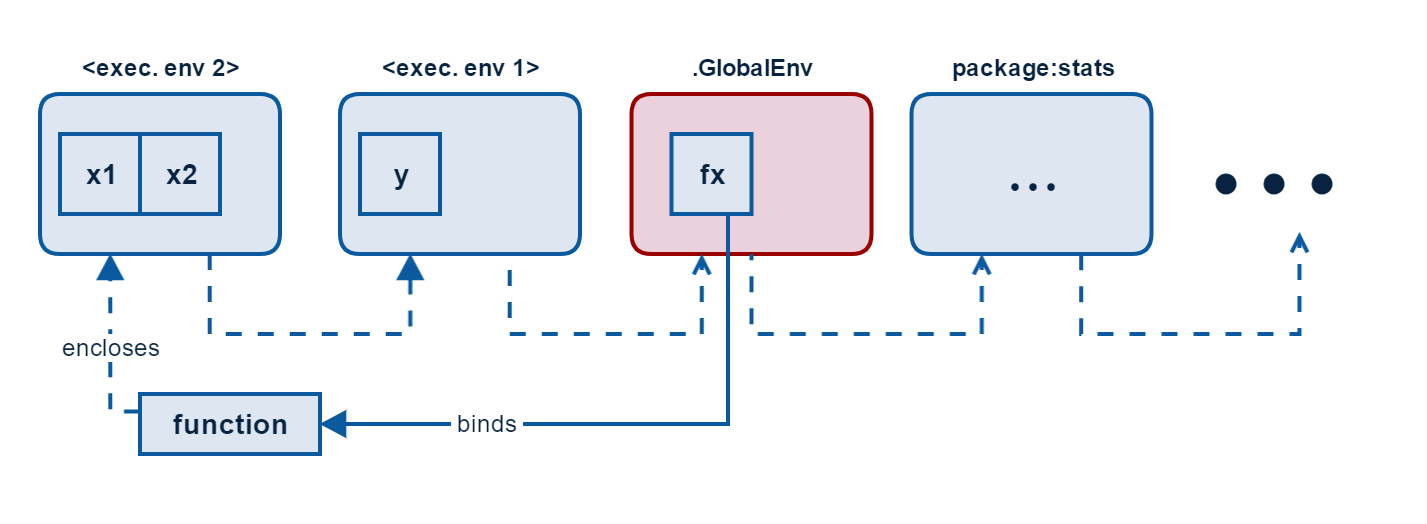
\includegraphics[width=\textwidth]{img/func-exec.png}

\subsection{Possible ways of serializing the environments}
There are two possible ways of serializing environments that differs in the way they treat symbols, that exist in the enclosing environment, but we cannot say for sure, whether the function is going to use them. Serializing the whole hierarchy serializes them, but serializing into a simplified environment does not.

\subsubsection{Serializing the whole hierarchy of environments}
The serialization could start in the enclosing environment of function \verb|fx| and then continue recursively into the parent environment until it reaches the environment of the first package and stops there. When serializing an environment, it would serialize all the variables bound inside it and the result would be a tree of environments, that when deserialized and evaluated would recreate the original context of \verb|fx|. This process would have to check for loops and ensure each environment gets serialize only once. The advantage of this approach is that it will serialize all the symbols, that function may theoretically access, not just symbols that are referenced from its body.

\subsubsection{Serializing subset of variables into a simplified environment}
Another way is to reuse the idea used for serializing function arguments. Genthat could extract all the variables used inside the closure, look them up in the environment hierarchy and then extract them to a new environment (called simple environment) and serialize it.

The advantage of this method is that variables that are not necessary used within the closure will not be serialized, so the tests would be both smaller and more readable as they would not contain unused items.

\subsection{Chosen solution}
For the advantages mentioned in the last paragraph I have chosen to try the second approach. There are few improvements to it that I have come up with during implementation: First the variables are only captured when they came from environment preceding the first named environment or the global environment. This is done to prevent serialization functions and variables from packages, which is not necessary. Second is that the first named environment is captured, because it is going to be used as a parent environment to the simple environment containing the referenced variables. The goal is for function \verb|fx|, which uses (e.g) \verb|x2| from \verb|<exec. env2>| and \verb|y| from \verb|<exec. env1>| to create an environment containing both variables and referencing to \verb|.GlobalEnv| as its parent. 

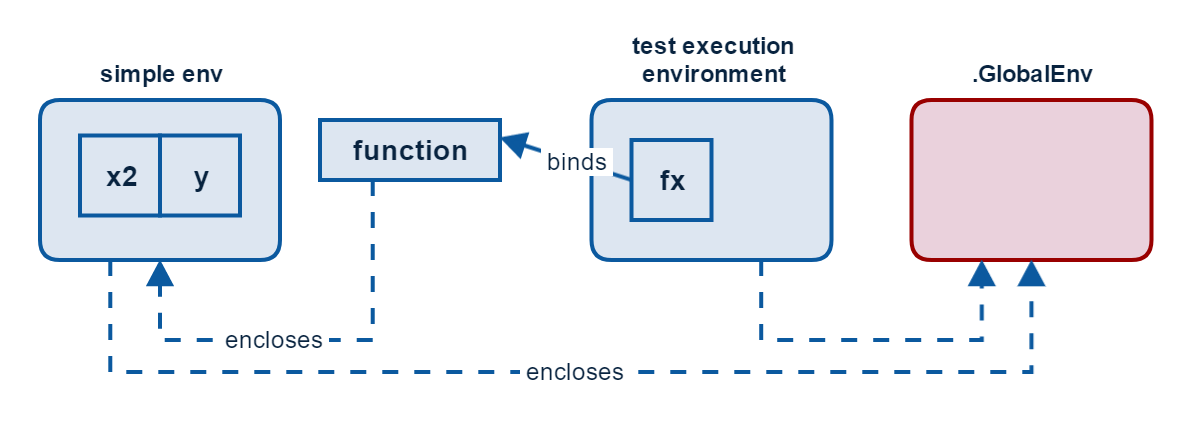
\includegraphics[width=\textwidth]{img/simple-env.png}

The diagram also contains test execution environment which is the execution environment of \verb|test_that| function call.

\subsubsection{Example}

If the body of \verb|fx| would contain just the symbols \verb|x1| and \verb|y| (just for brevity of the example) and we would pass it into the function called \verb|func| the generated test would look like this:

\begin{minted}{r}
test_that("fx", {
    # expected return value
    expected <- TRUE

    # closures
    fx <- function ()
    {
        x1
        y
    }
    `__fx_env` <- as.environment(list(x2 = 10L, y = "Hi!"))
    parent.env(`__fx_env`) <- .GlobalEnv
    environment(fx) <- `__f_env`

    expect_equal(func(fx), expected)
})
\end{minted}

\subsection{Serialization}
Now we have the simple environment and its parent. Next step is to extract the formals of the closure and its body. These four parts together make a list, that contains our deconstructed closure. This list is then assigned to a name \verb|fx| inside another list, containing all the closures generated from one trace (in traces this list is named \verb|cls|).

When the serialization happens, Genthat serializes the body as an expression (so it would not get wrapped in quote) and the rest uses the same serialization as any other variable value.

\subsection{Test generation}
From the list containing four strings with snippets of R code Genthat has to generate the closure for the test case. First it assembles back the closure and parses it. This is done for pretty printing the closure, because the R’s native \verb|deparse| function handles the formatting better. We could use only the \verb|deparse| function for serializing the closure, but that would lead to loss of precision when serializing numerical values inside the closure, that is why we first use our custom serialization and then again serialize it with R’s function.

Second step is to assemble the call to create the simple environment, set its parent and set simple environment as the enclosing environment for the closure.

Closure is now recreated and when test case calls \verb|fx|, everything should execute as expected.

\subsubsection{Example}
Now when we can combine few of the previous examples and show how test generation works for them after all the improvements have been implemented. 

We are going to use the \verb|lapply2| function from the introduction and the \verb|mod_adder| from the chapter \ref{ssec:clos1} about closures.

\begin{minted}{r}
lapply2 <- function(x, f, ...) {
  out <- vector("list", length(x))
  for (i in seq_along(x)) {
    out[[i]] <- f(x[[i]], ...)
  }
  out
}
mod_adder <-function(mod)function(a, b) { (a + b) %% mod }
add13 <- mod_adder(13L)
vals <- list(40L, 24L, 4L, 19L)  
lapply2(vals, function(x) add13(10L,x))
\end{minted}

From the last function call the following test can be generated:

\begin{minted}{r}
test_that("lapply2", {                   
    # expected return value   
    expected <- list(11L,21L,14L,16L)        
    
    # variables used in arguments                     
    vals <- list(40L, 24L, 4L, 19L)
    
    # closures                     
    add13 <- function (a, b)
    {
        (a + b)%%mod
    }
    `__add13_env` <- as.environment(list(mod = 13L))
    parent.env(`__add13_env`) <- .GlobalEnv
    environment(add13) <- `__add13_env`
    
    expect_equal(lapply2(vals, function(x) add13(10L,x)), expected)
})                               
\end{minted}

\setsecnumdepth{part}
\chapter{Conclusion}
This thesis has described many nuances the R language has in the context of closures and expression evaluation, it explained how Genthat may improve existing R code and how it works inside. The main goal of this thesis has been to implement serialization of closures, I believe that it has been reached and although there may be some rough edges or bugs waiting to be discovered, it laid a foundation to build upon. 


\section{Future work}
As of finishing this thesis, Genthat has been undergoing a refactoring to integrate all the new features and simplify future development. After it is done, it should be possible to run it on the CRAN repository and use the result to choose in which areas should the future work take place.

One of the possible improvements may be tracing changes in the enclosing environments, so Genthat could also generate tests to track side effects of functions. Or using the binary form only for numbers, that are going to be affected by the precision loss and not for all real numbers.


\bibliographystyle{iso690}
\bibliography{mybibliographyfile}

\setsecnumdepth{all}
\appendix

\chapter{Contents of enclosed CD}

%change appropriately

\begin{figure}
	\dirtree{%
		.1 readme.txt\DTcomment{the file with CD contents description}.
		.1 src\DTcomment{the directory of source codes}.
		.2 genthat\DTcomment{pre-cloned directory with latest Genthat sources}.
		.2 thesis\DTcomment{the directory of \LaTeX{} source codes of the thesis}.
		.3 img\DTcomment{diagrams and graphs from the thesis}.
		.1 text\DTcomment{the thesis text directory}.
		.2 BP\_Vacha\_Michal\_2017.pdf\DTcomment{the thesis text in PDF format}.
	}
\end{figure}

\end{document}
